\subsection{Ca sử dụng tra cứu du lịch}
\vspace{0.5cm}


\noindent 
\begin{tabularx}{\linewidth}{| l | X |} 
\hline 
\textbf{Mô tả} & Người dùng tra cứu và lọc tên địa điểm du lịch, sự kiện, điểm đến muốn tìm hiểu.  \\ 
\hline 
\textbf{Luồng cơ bản} & 1. Người dùng truy cập tab khám phá và bấm vào thanh tìm kiếm \newline
                       2. Hệ thống hiển thị lịch sử tìm kiếm và các bộ lọc. \newline
                       3. Người dùng nhập từ khóa tìm kiếm. \newline
                       4. Hệ thống tra lưu từ khóa tìm kiếm và hiện thị kết quả theo danh sách. \\
\hline 
\textbf{Luồng thay thế} & Người dùng tìm kiếm và chọn bộ lọc (sự kiện, địa điểm, nhà hàng, khách sạn, điểm đến,...).\\
                         
\hline 
\textbf{Tiền điều kiện} & Người dùng đang đăng nhập và phiên đăng nhập chưa kết thúc. \\
\hline 
\textbf{Hậu điều kiện} & - Người dùng có thể xem thông tin về các kết quả tìm kiếm.\newline
                         - Hệ thống lưu lại lịch sử tìm kiếm của người dùng. \newline
                         - Hệ thống cập nhật sở thích của người dùng. \\

\hline 
\textbf{Yêu cầu phi chức năng} & Hệ thống xử lý tìm kiếm không quá 2s  \\ 
\hline 
\end{tabularx}

\vspace{0.8cm}

\noindent 
\begin{tabular}{| c | c |}
    \hline
    \textbf{Biểu đồ hoạt động} & \textbf{Quan hệ} \\ 
    \hline
    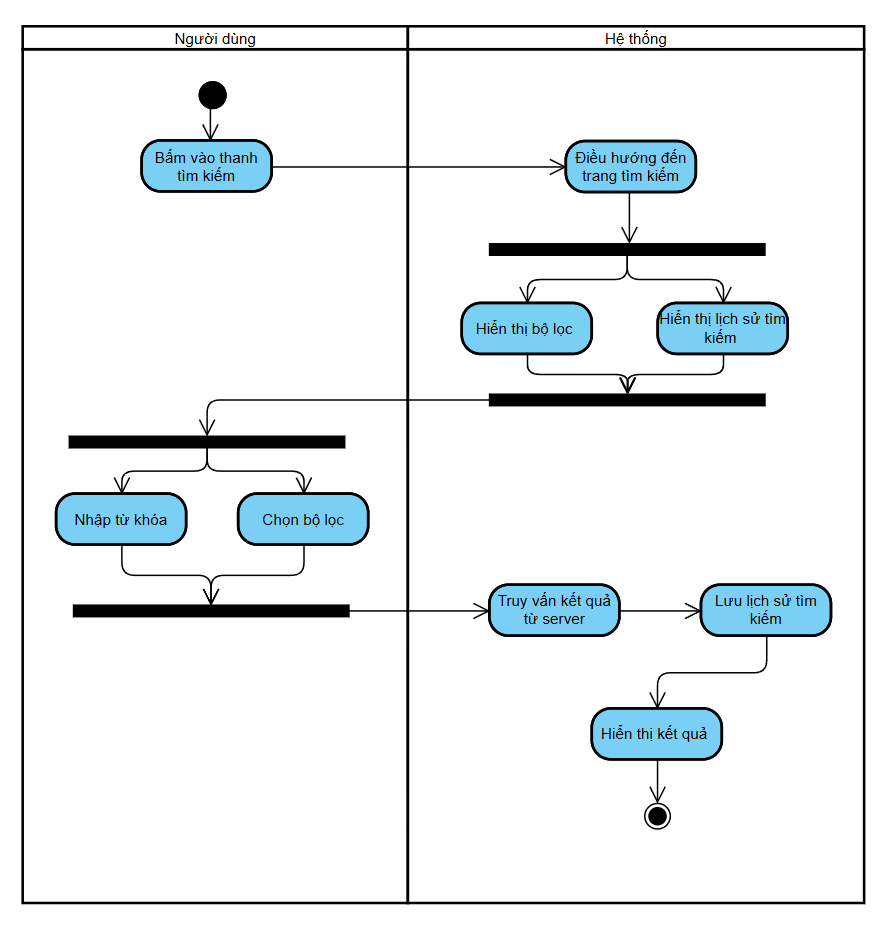
\includegraphics[width=0.5\linewidth]{figures/c3/3-3-5-ad.png} 
    & 
    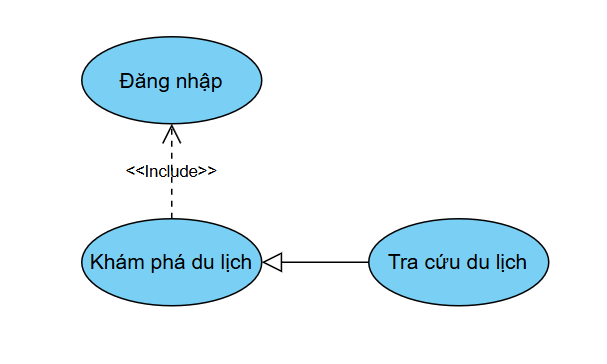
\includegraphics[width=0.45\linewidth]{figures/c3/3-3-5-rd.png} \\ 
    \hline
\end{tabular}



\begin{figure}[H]
    \centering  
    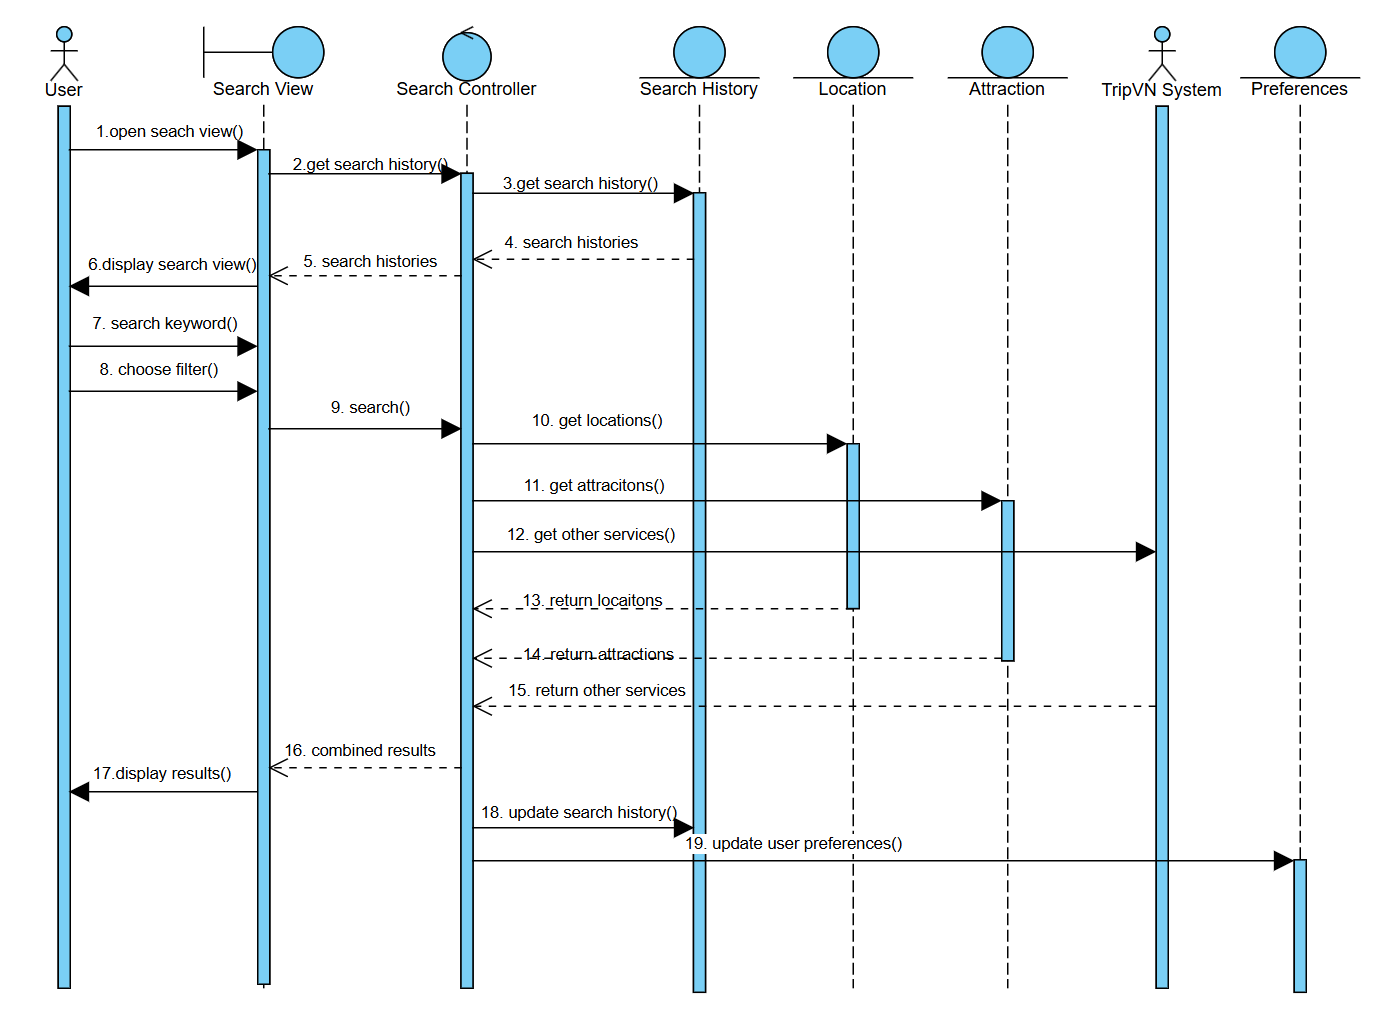
\includegraphics[width=1\textwidth]{figures/c3/3-3-5-sd.png}
    \caption{Biểu đồ tuần tự ca sử dụng tra cứu du lịch.}
    \label{fig:3-3-5-sequence-diagram}
\end{figure}